\chapter{Discussão}
De maneira geral, podemos ver a clara diferença que faz escolher um algoritmo de ordenação ideal, sendo dos 7 analisados, apenas 3 bons o suficiente para uso com arranjos grandes. Pode-se também notar que a escolha do algoritmo não faz tanta diferença se considerarmos arranjos de apenas 100 elementos ou menores, como pode ser visto nos gráficos seguintes:

\begin{figure}[H]
	\centering
	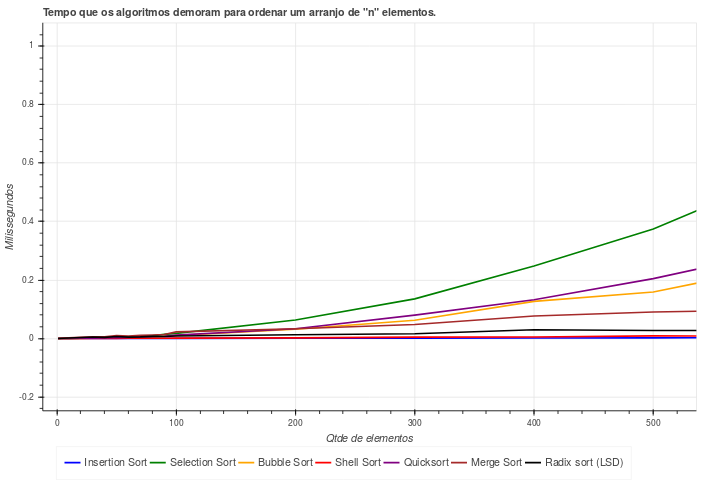
\includegraphics[scale=0.6]{img/igualdade/aleatorios.png}
	\caption{Gráfico de resultados para arranjos com os 100 primeiros elementos aleatórios.}
	\label{graph-aleatorio-comp}
\end{figure}

\begin{figure}[H]
	\centering
	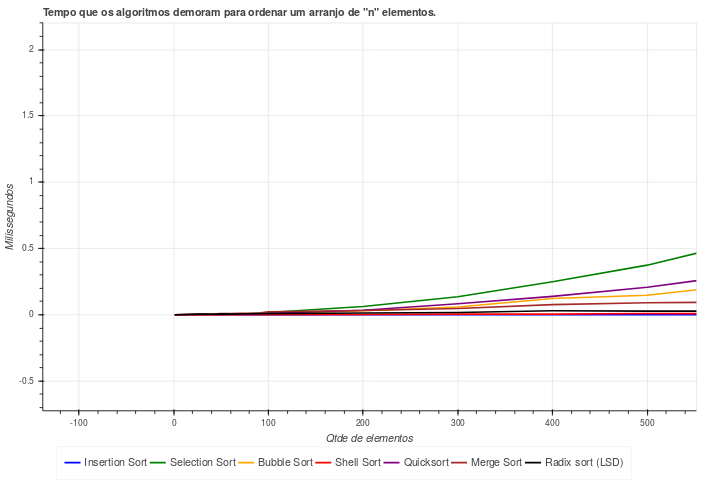
\includegraphics[scale=0.6]{img/igualdade/crescentes.png}
	\caption{Gráfico de resultados para arranjos com os 100 primeiros elementos em ordem crescente.}
	\label{graph-crescente-comp}
\end{figure}

\begin{figure}[H]
	\centering
	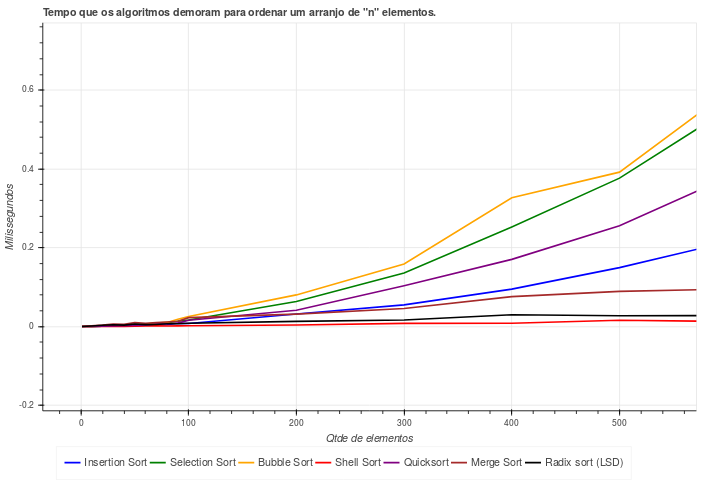
\includegraphics[scale=0.6]{img/igualdade/decrescentes.png}
	\caption{Gráfico de resultados para arranjos com os 100 primeiros elementos em ordem decrescente.}
	\label{graph-decrescente-comp}
\end{figure}

Dos 7, o algoritmo mais recomendado para uso é o \texttt{Shell sort}, pois no seu pior caso (ordem decrescente dos elementos) ele obteve uma média de $3.3127751999999986$ milissegundos, enquanto o segundo melhor algoritmo, \texttt{Radix sort (LSD)}, obteve $5.770450800000001$, pouco mais de dois milissegundos de diferença.

Mesmo sendo o segundo melhor algoritmo desse estudo, o \texttt{Radix sort (LSD)} mostrou-se ser muito superior a grande parte dos algoritmos de ordenação que utilizam comparação de chaves, visto que o \texttt{Radix} utiliza a decomposição das chaves.

Observando os valores dos algoritmos que utilizam recursão, \texttt{Quicksort} e \texttt{Merge sort}, podemos ver que o \texttt{Quick} é melhor se comparado ao \texttt{Merge} na ordenação dos arranjos de 100 elementos ou menores. Porém, o \texttt{Merge} mostrou-se ser bastante mais eficaz que o \texttt{Quick} a medida que a quantidade de elementos nos arranjos ia subindo, possuindo uma diferença entre seus piores casos de 9090 segundos.

Algo interessante a se notar, é a aproximação dos resultados quanto comparado os valores para arranjos aleatórios e arranjos crescentes, havendo uma diferença mais significante quanto comparado com os valores para arranjos decrescentes (piores casos).